In this section we consider the random tie-breaking rule. 
%We present a series of single threshold strategies, analyze their guarantees and show matching lower bounds.

We start by establishing a series of single threshold strategies that guarantee high utilities.
\begin{theorem}
		\label{thm:prophet_threshold_inequality}
		For every $\ell=1, \ldots, n$, let $T^\ell = \frac{1}{k+\ell}\sum_{j=1}^{\ell} \E [y_j]$. 
		Then, for every agent, the single threshold strategy $T^{\ell}$ (i.e., select $v_t$ iff $v_t\geq T^\ell$) guarantees an expected utility of at least $T^{\ell}$.
\end{theorem}	
\begin{proof}
	Fix an agent $i$. Let $S_{-i}$ be the strategies of all agents except agent $i$, and let $S=(T^\ell,S_{-i})$.
	Let $\assignn{i}{j}{S}$ denote the event that agent $i$ is assigned the reward $v_j$ in strategy profile $S$. I.e., $\assignn{i}{j}{S}$ is the event that agent $i$ competed over reward $v_j$ and received it according to the random tie-breaking rule. 
	For simplicity of presentation, we omit $S$ and write $\assign{i}{j}$.
	It holds that
%%	\begin{eqnarray*}
%\[		 u_i(S)  =
%		 \E\left[ \sum_{j=1}^{n}{v_j\cdot \Pr\left(\assign{i}{j}\right)}\right] =  \]
%\[ 		  \E\left[\sum_{j=1}^{n}{(T^\ell+v_j-T^\ell) \Pr\left(v_j\geq T^\ell,\forall_{r<j}  \overline{\assign{i}{r}},\assign{i}{j}\right)}\right]. \nonumber\]
%%	\end{eqnarray*}

\begin{eqnarray*}
	 u_i(S)  & = & \E\left[ \sum_{j=1}^{n}{v_j\cdot \Pr\left(\assign{i}{j}\right)}\right]\\
	& = & \E\left[\sum_{j=1}^{n}{(T^\ell+v_j-T^\ell) \Pr\left(v_j\geq T^\ell,\forall_{r<j}  \overline{\assign{i}{r}},\assign{i}{j}\right)}\right].
\end{eqnarray*}

Let $p=\sum_{j=1}^{n} \Pr(v_j\geq T^\ell,\forall_{j'<j}  \overline{\assign{i}{j'}},\assign{i}{j})$ (i.e., $p$ is the probability that agent $i$ receives some reward in strategy profile $S=(T^{\ell},S_{-i})$), and let $Z^{+}=\max\{Z,0\}$.
We can now write $u_i(S)$ as follows:
\begin{eqnarray*}
	u_i(S) 	& =  &p T^\ell + \E\left[\sum_{j=1}^{n}{(v_j-T^\ell)^+\Pr\left(\forall_{r<j}\overline{\assign{i}{r}},\assign{i}{j}\right)}\right]  \nonumber\\
	 &= & p\cdot T^\ell  + \E\Bigl[\sum_{j=1}^{n}(v_j-T^\ell)^+ \cdot \Pr\left(\forall_{r<j}\overline{\assign{i}{r}} \right)   \cdot\Pr\left(\assign{i}{j} \mid \forall_{r<j}\overline{\assign{i}{r}}\right)\Bigr] \nonumber\\
	 &\geq &	 p\cdot T^\ell + \E\Bigl[\sum_{j=1}^{n}(v_j-T^\ell)^+\cdot (1-p) \Bigr. \left. \cdot \Pr\left(\assign{i}{j} \mid \forall_{r<j}\overline{\assign{i}{r}}\right)\right] \nonumber\\
	 &\geq  &  p\cdot T^\ell +\frac{1-p}{k}\cdot \E\left[\sum_{j=1}^{n}(v_j-T^\ell)^{+}\right]. \nonumber 
\end{eqnarray*}		
The first inequality holds since the probability of not getting any reward until time $j$ is bounded by $1-p$ (i.e., the probability of not getting any reward). 
The last inequality holds since if $v_j-T^\ell\geq 0$ and agent $i$ is still active, the reward is selected, thus assigned with probability at least $1/k$. 
Since each term in the summation is non-negative, we get the following:
%After removing any smaller term, we further remove the non-negativity demand and, again, can only decrease the total sum. Hence,
\begin{eqnarray*}		
%		& = & p\cdot T^\ell +\frac{1-p}{k}\cdot \E\left[\sum_{j=1}^{n}(y_j-T^\ell)^{+}\right] \nonumber \\ 
	u_i(S)	& \geq & p\cdot T^\ell +\frac{1-p}{k}\cdot \E\left[\sum_{j=1}^{\ell}(y_j-T^\ell)^{+}\right] \nonumber \\ 
		& \geq  &p\cdot T^\ell + \frac{1-p}{k}\cdot \E\left[\sum_{j=1}^{\ell}y_j-\ell\cdot  T^\ell\right] \nonumber\\
		& =  &p\cdot T^\ell + \frac{1-p}{k}\cdot \left((k+\ell)\cdot T^\ell-\ell \cdot T^\ell\right)  = T^{\ell},\nonumber
\end{eqnarray*}
where the last equality follows by the definition of $T^\ell$.
\end{proof}

The special cases of $\ell=1$ and $\ell=k$ give the following corollaries:
\begin{corollary}
	The single-threshold strategy $T^k$ guarantees an expected utility of at least $\frac{1}{2k}\E[\sum_{i=1}^{k}y_i]$. 
\end{corollary}
\begin{corollary}
	The single-threshold strategy $T^1$ guarantees an expected utility of at least $\frac{1}{k+1}\E[y_1]$.
\end{corollary}

We now show that the bound in Theorem~\ref{thm:prophet_threshold_inequality} is tight.
\begin{proposition}\label{pro:lb_random}
	For every $\epsilon>0$ there exists an instance such that in the unique equilibrium of the game, no agent gets an expected utility of more than  $\frac{1}{k+\ell}\sum_{j=1}^{\ell} \E [y_j]+\epsilon$ for any $\ell \leq n$.
\end{proposition}
\begin{proof}
	Given an $\epsilon>0$, consider the following instance (depicted in Figure~\ref{fig:random}): 
	$$
	v_t=1 \mbox{ for all } t\leq n-1, ~\mbox{  and  }~  v_n=\begin{cases}
	\frac{k+\epsilon}{\epsilon} & \text{ w.p. } \epsilon\\
	0 & \text{ w.p. } 1-\epsilon
	\end{cases}
	$$
	One can easily verify that in the unique equilibrium $S$, all agents compete over the last reward, for an expected utility of 	 $1+\frac{\epsilon}{k}$. 
	It holds that for every agent $i$:
	$$u_i(S) =  1+\frac{\epsilon}{k} \leq 1+\epsilon =  
	%\frac{\ell+ \epsilon \left(\frac{k+\epsilon}{\epsilon}-1\right)}{k+\ell}+\epsilon= 
	\frac{\E[\sum_{j=1}^{\ell}y_j]}{k+\ell}+\epsilon.$$
	This example also shows that there are instances in which the social welfare in equilibrium is at most half the optimal welfare allocation. 
\end{proof}

\begin{figure}[h!]
	\centering
	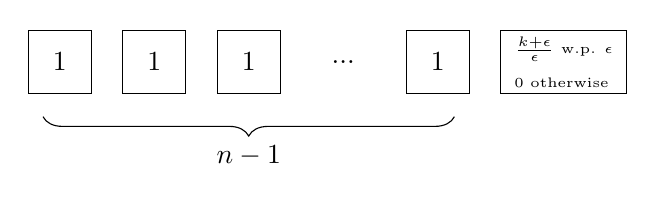
\begin{tikzpicture}[scale=0.4]
	\draw (0,0) rectangle node (C) {$1$} ++(2,2); 
	\draw (3,0) rectangle node (D) {$1$} ++(2,2); 
	%\draw (6,0) rectangle node (E) {$1$} ++(2,2); 
	\draw (6,0) rectangle node (F) {$1$} ++(2,2); 
	\draw [draw=white](9,0) rectangle node (dots) {...} ++(2,2); 
	\draw (12,0) rectangle node (A) {$1$} ++(2,2); 
	\draw (15,0) rectangle node (B)[align=left] {\tiny$\frac{k+\epsilon}{\epsilon}$ w.p. $\epsilon$\\\tiny$0$ otherwise} ++(4,2); 
	\draw[decorate,decoration={brace, amplitude=7pt, raise=13pt, mirror}]
	(C.south west) to node[black,below= 20pt] {$n-1$} (A.south east);%
	\end{tikzpicture}
	\caption{An example where the expected reward is no more than $\frac{1}{k+\ell}\sum_{j=1}^{\ell} \E [y_j]+\epsilon$}
	\label{fig:random}
\end{figure}


